%%%%%%%%%%%%%%%%%%%%%%%%%%%%%%%%%%%%%%%%%
% Beamer Presentation
% LaTeX Template
% Version 1.0 (10/11/12)
%
% This template has been downloaded from:
% http://www.LaTeXTemplates.com
%
% License:
% CC BY-NC-SA 3.0 (http://creativecommons.org/licenses/by-nc-sa/3.0/)
%
%%%%%%%%%%%%%%%%%%%%%%%%%%%%%%%%%%%%%%%%%

%----------------------------------------------------------------------------------------
% PACKAGES AND THEMES
%----------------------------------------------------------------------------------------

\documentclass[table, xcolor={dvipsnames}, 9pt]{beamer}
\usepackage{tikz}
\usetikzlibrary{positioning}
\mode<presentation> {

% The Beamer class comes with a number of default slide themes
% which change the colors and layouts of slides. Below this is a list
% of all the themes, uncomment each in turn to see what they look like.

%\usetheme{default}
%\usetheme{AnnArbor}
%\usetheme{Antibes}
%\usetheme{Bergen}
%\usetheme{Berkeley}
%\usetheme{Berlin}
%\usetheme{Boadilla}
%\usetheme{CambridgeUS}
%\usetheme{Copenhagen}
%\usetheme{Darmstadt}
%\usetheme{Dresden}
%\usetheme{Frankfurt}
%\usetheme{Goettingen}
%\usetheme{Hannover}
%\usetheme{Ilmenau}
%\usetheme{JuanLesPins}
%\usetheme{Luebeck}
% \usetheme{Madrid}
\usetheme{metropolis}
%\usetheme{Malmoe}
%\usetheme{Marburg}
%\usetheme{Montpellier}
%\usetheme{PaloAlto}
%\usetheme{Pittsburgh}
%\usetheme{Rochester}
%\usetheme{Singapore}
%\usetheme{Szeged}
%\usetheme{Warsaw}

% As well as themes, the Beamer class has a number of color themes
% for any slide theme. Uncomment each of these in turn to see how it
% changes the colors of your current slide theme.

%\usecolortheme{albatross}
%\usecolortheme{beaver}
%\usecolortheme{beetle}
%\usecolortheme{crane}
%\usecolortheme{dolphin}
%\usecolortheme{dove}
%\usecolortheme{fly}
%\usecolortheme{lily}
%\usecolortheme{orchid}
%\usecolortheme{rose}
%\usecolortheme{seagull}
%\usecolortheme{seahorse}
%\usecolortheme{whale}
%\usecolortheme{wolverine}

%\setbeamertemplate{footline} % To remove the footer line in all slides uncomment this line
%\setbeamertemplate{footline}[page number] % To replace the footer line in all slides with a simple slide count uncomment this line

%\setbeamertemplate{navigation symbols}{} % To remove the navigation symbols from the bottom of all slides uncomment this line
}

\usepackage{graphicx} % Allows including images
\usepackage{booktabs} % Allows the use of \toprule, \midrule and \bottomrule in tables
\usepackage{multirow}
\usepackage{natbib}
\usepackage[]{hyperref}
\usepackage{diagbox}
\usepackage{makecell}
\usepackage{subfig}
\usepackage{amsmath}
\usepackage{amsfonts,amsthm,amsmath,amssymb}    
\usepackage{bbm}
\usepackage{bm}
\usepackage{empheq}

\hypersetup{unicode=true,
            pdfusetitle,
            bookmarks=true,
            bookmarksnumbered=true,
            bookmarksopen=true,
            bookmarksopenlevel=2,
            breaklinks=false,
            pdfborder={0 0 1},
            backref=true,
            hypertexnames=false,
            pdfstartview={XYZ null null 1}}
\usepackage{xcolor}
\newcommand\myheading[1]{%
  \par\bigskip
  {\Large\bfseries#1}\par\smallskip}
\newcommand\given[1][]{\:#1\vert\:}
\theoremstyle{newstyle}
\newtheorem{thm}{Theorem}
\newtheorem{prop}[thm]{Proposition}
\newtheorem{lem}{Lemma}
\newtheorem{cor}{Corollary}
\newtheorem{defin}{Definition}
\newcommand*\diff{\mathop{}\!\mathrm{d}}
\newcommand*\Diff[1]{\mathop{}\!\mathrm{d^#1}}
\newcommand*{\QEDA}{\hfill\ensuremath{\blacksquare}}%
\newcommand*{\QEDB}{\hfill\ensuremath{\square}}%
\DeclareMathOperator{\E}{\mathrm{E}}
\DeclareMathOperator{\R}{\mathbb{R}}
\DeclareMathOperator{\Var}{\rm{Var}}
\DeclareMathOperator{\Cov}{\rm{Cov}}
\DeclareMathOperator{\e}{\rm{e}}
\DeclareMathOperator{\logit}{\rm{logit}}
\DeclareMathOperator{\indep}{{\perp\!\!\!\perp}}
%\DeclareMathOperator{\Pr}{\rm{Pr}}
\newenvironment{Column}[1][.5\linewidth]{\begin{column}{#1}}{\end{column}}
%----------------------------------------------------------------------------------------
% TITLE PAGE
%----------------------------------------------------------------------------------------

\title[]{Estimation of Average Causal Effects} % The short title appears at the bottom of every slide, the full title is only on the title page

\author{Thomas Leavitt} % Your name
\institute[] % Your institution as it will appear on the bottom of every slide, may be shorthand to save space
{
% Your institution for the title page
\medskip
\textit{} % Your email address
}
\date{\today} % Date, can be changed to a custom date

\begin{document}

\begin{frame}
\titlepage % Print the title page as the first slide
\end{frame}

%\begin{frame}
%\frametitle{Overview} % Table of contents slide, comment this block out to remove it
%\tableofcontents % Throughout your presentation, if you choose to use \section{} and \subsection{} commands, these will automatically be printed on this slide as an overview of your presentation
%\end{frame}

%------------------------------------------------------------------------
% PRESENTATION SLIDES
%------------------------------------------------------------------------
\section{The average treatment effect}
\begin{frame}
\frametitle{Average treatment effect: An example} 

\begin{itemize}
\item Consider the ``village heads'' study from Gerber and Green (Chapter 2): 
\item[]
\begin{center}
\begin{tabular}{l|rrr} \hline
& \multicolumn{3}{c}{Budget share (\%)} \\
Village &$y_{c}$& $y_{t}$& $\tau$  \\ \hline
1& 10 & 15  & 5  \\
2& 15 & 15  & 0   \\ 
3& 20 & 30  & 10   \\
4& 20 & 15  & -5   \\
5& 10 & 20  & 10   \\
6& 15 & 15  & 0   \\
7& 15 & 30  & 15   \\ \hline
Average & 15 & 20 & 5  \\ \hline
\end{tabular}
\end{center}
\item[]
\item The target of interest is the \textit{average treatment effect}:
\begin{align*}
\bar{\tau} & = \frac{1}{n}\sum \limits_{i = 1}^{n} \left(y_{ti} - y_{ci}\right) = \frac{1}{n}\sum \limits_{i = 1}^{n} \tau_i
\end{align*}
\end{itemize}
\end{frame}
%------------------------------------------------------------------------
\begin{frame}
\frametitle{Estimation: An example} 
\begin{itemize}
\item Imagine a randomized experiment in which the realized data are as follows: 
\item[]
\begin{center}
\begin{tabular}{lr|rrr} \hline
& & \multicolumn{3}{c}{Budget share (\%)} \\
Village & $z$ & $y_{c}$& $y_{t}$& $\tau$  \\ \hline
1& 1 & ?  & 15  & ?  \\
2& 0 & 15 & ?   & ?   \\ 
3& 0 & 20 & ?   & ?   \\
4& 0 & 20 & ?   & ?   \\
5& 0 & 10 & ?   & ?   \\
6& 0 & 15 & ?   & ?   \\
7& 1 & ?  & 30  & ?   \\ \hline
 & Average & 16 & 22.5 & 6.5  \\ \hline
\end{tabular}
\end{center}
\item[]
\item \textit{Difference-in-Means} \textbf{estimate} for this particular realized assignment is $6.5$
\item We are going to show that the \textit{expected value} of the \textbf{estimator} over all possible assignments is equal to $\bar{\tau}$
\end{itemize}
\end{frame}
%------------------------------------------------------------------------
\section{Estimator of average treatment effect}
\begin{frame}
\frametitle{Difference-in-Means estimator} 
\begin{itemize}
\item Define the Difference-in-Means estimator as follows: 
\begin{itemize}
\item When the number of treated units, $n_1$, is fixed:
\begin{align*}
\hat{\bar{\tau}}\left(\mathbf{Z}, \mathbf{Y}\right) & = \frac{1}{n_1}\mathbf{Z}'\mathbf{Y} - \frac{1}{n_0}\left(\mathbf{1} - \mathbf{Z}\right)'\mathbf{Y} \\ 
& = \frac{1}{n_1}\sum \limits_{i = 1}^n Z_i Y_i - \frac{1}{n_0}\sum \limits_{i = 1}^n \left(1 - Z_i\right) Y_i,
\end{align*}
where $Y_i = Z_i y_{ti} + \left(1 - Z_i\right)y_{ci}$
\item When the number of treated units, $\mathbf{Z}'\mathbf{1}$, is random:
\begin{align*}
\hat{\bar{\tau}}\left(\mathbf{Z}, \mathbf{Y}\right) & = \frac{\mathbf{Z}'\mathbf{Y}}{\mathbf{Z}'\mathbf{1}} - \frac{\left(\mathbf{1} - \mathbf{Z}\right)'\mathbf{Y}}{\left(\mathbf{1} - \mathbf{Z}\right)'\mathbf{1}} \\ 
& = \cfrac{\sum \limits_{i = 1}^n Z_i Y_i}{\sum\limits_{i = 1}^n Z_i} - \frac{\sum \limits_{i = 1}^n \left(1 - Z_i\right) Y_i}{\sum \limits_{i = 1}^n \left(1 - Z_i\right)}
\end{align*}
\end{itemize}
\end{itemize}
\end{frame}
%------------------------------------------------------------------------
\begin{frame}
\frametitle{Difference-in-Means estimator} 
\begin{itemize}
\item First consider complete random assignment (fixed $n_1$): 
\begin{itemize}
\item $2$ out of $7$ villages are assigned to treatment and the remaining $5$ are assigned to control
\item There are $\binom{7}{2} = 21$ possible assignments:
\begin{equation*}
  \Omega =
  \left\{
    \begin{bmatrix} 1 \\ 1 \\ 0 \\ 0 \\ 0 \\ 0 \\ 0 \end{bmatrix},
    \begin{bmatrix} 1 \\ 0 \\ 1 \\ 0 \\ 0 \\ 0 \\ 0 \end{bmatrix},
    \cdots ,
    \begin{bmatrix} 0 \\ 0 \\ 0 \\ 0 \\ 0 \\ 1 \\ 1 \end{bmatrix}
  \right\}.
\end{equation*}
\end{itemize}
\end{itemize}
\end{frame}
%------------------------------------------------------------------------
\begin{frame}
\frametitle{Difference-in-Means estimator} 
\begin{itemize}
 \item There are $\binom{7}{2} = 21$ possible realization of data corresponding to the $\binom{7}{2} = 21$ possible assignments:
 \item[]
 \item[]
\begin{table}[H]
\scriptsize
    \begin{tabular}{l|l|l|l|}
    $\mathbf{z}_1$ & $\mathbf{y_c}$ & $\mathbf{y_t}$ & $\mathbf{y}_1$ \\ \midrule
    1 & ?  & 15  & 15 \\
    1 & ?  & 15  & 15 \\
    0 & 20 & ?   & 20 \\
    0 & 20 & ?   & 20 \\
    0 & 10 & ?   & 10 \\
    0 & 15 & ?   & 15 \\
    0 & 15 & ?   & 15 \\
    \end{tabular}
    \hfill
      \begin{tabular}{l|l|l|l|}
    $\mathbf{z}_2$ & $\mathbf{y_c}$ & $\mathbf{y_t}$ & $\mathbf{y}_2$ \\ \midrule
    1 &  ? & 15 & 15 \\
    0 & 15 & ?  & 15 \\
    1 & ?  & 30 & 30 \\
    0 & 20 & ?  & 20 \\
    0 & 10 & ?  & 10 \\
    0 & 15 & ?  & 15 \\
    0 & 15 & ?  & 15 \\
    \end{tabular}
     \hfill
     $\cdots $
     \hfill
      \begin{tabular}{l|l|l|l|}
    $\mathbf{z}_{21}$ & $\mathbf{y_c}$ & $\mathbf{y_t}$ & $\mathbf{y}_{21}$ \\ \midrule
    0 & 10 & ?  & 10 \\
    0 & 15 & ?  & 15 \\
    0 & 20 & ?  & 20 \\
    0 & 20 & ?  & 20 \\
    0 & 10 & ?  & 10 \\
    1 & ?  & 15 & 15 \\
    1 & ?  & 30 & 30 \\
    \end{tabular}
\end{table}
\item[]
\item The random vectors of $\mathbf{Z}$ and $\mathbf{Y}$ can take on any of the possible values, $\left(\mathbf{z}_1, \mathbf{y}_1\right), \cdots , \left(\mathbf{z}_{21}, \mathbf{y}_{21}\right)$, given in the table above.
\item If we apply the Difference-in-Means estimator to the $21$ possible realizations of data in the table, then there are $21$ possible estimates that correspond to each of the $21$ possible realizations of data:
\begin{equation*}
\hat{\bar{\tau}}\left(\mathbf{z}_1, \mathbf{y}_1\right) = -1, \, \hat{\bar{\tau}}\left(\mathbf{z}_2, \mathbf{y}_2\right) = 7.5, \, \cdots \, , \, \hat{\bar{\tau}}\left(\mathbf{z}_{21}, \mathbf{y}_{21}\right) = 7.5
\end{equation*}
\end{itemize}
\end{frame}
%------------------------------------------------------------------------
\section{Review of expected value}
\begin{frame}{Review of expectations}
\frametitle{}
  \begin{itemize}
  \item Consider arbitrary \textit{random variables} $V$, $W$.
  \item (For simplicity, assume discrete --- as $\mathbf{Z}$ generally is.)
  \item  $\E(V) = \sum_{\mbox{all v's}} v\Pr(V=v) $.
  \item For constant $\alpha$, $\E \left[\alpha\right] = \alpha$
  \item For constants $\alpha, \beta$, $\E \left[\alpha + \beta V\right] = \alpha + \beta\E\left[V\right]$.
  \item Also $\E\left[\alpha V + \beta W)\right] = \alpha \E\left[V\right] + \beta \E\left[W\right]$. 
  \item In particular, 
  \begin{align*}
\E\left(\frac{1}{n} \sum_{i=1}^n V_i\right) & \\
& = \E \left[\frac{1}{n} \left(V_1 + V_2 + \dots + V_n\right)\right] \\
& = \frac{1}{n}\E \left[V_1 + V_2 + \dots + V_n\right] \\ 
& = \frac{1}{n}\E \left[V_1\right] + \E\left[V_2\right] + \dots + \E\left[V_n\right] \\ 
& = \frac{1}{n} \sum_{i=1}^n \E \left[V_i\right] 
\end{align*}
  \end{itemize}
\end{frame}
%------------------------------------------------------------------------
\begin{frame}{Review of expectations}
\begin{itemize}
\item Matrices \& vectors: $(a_{1}, a_{2}, \ldots, a_{n})' = \left(
    \begin{array}{c}
      a_{1} \\ \vdots \\ a_{n}
    \end{array}
\right)$ ;  $\left(
      \begin{array}{c}
        b_{1} \\  \vdots \\ b_{n}\\
      \end{array}
\right)' = (b_{1}, \ldots, b_{n})$.
  \item By convention, $X, Y, Z$ denote random variables (RVs); $x, y, z$, realizations of the RVs.
 \item $x_{i}$= subject $i$ measurement; $\mathbf{x} =(x_{1}, \ldots, x_{n})'$ column of measurements
  \item $Z_i$= random variable for subject $i$; $\mathbf{Z}=(Z_1, Z_2,
    \ldots, Z_n)'$ (a ``random vector'').  
  \item So $\mathbf{z}=(z_1, z_2, \ldots, z_n)'$ denotes a particular
    realization of $\mathbf{Z} $.
  \item Vector cross products: $\mathbf{a}'\mathbf{b}  = a_{1}b_{1} + \cdots + a_{n}b_{n}$
  \end{itemize}
\end{frame}
%------------------------------------------------------------------------
\section{Unbiasedness of Difference-in-Means estimator}
\begin{frame}{Unbiasedness of Difference-in-Means estimator}

\begin{center}
Go to PDF of proof and to \texttt{R} . . . 
\end{center}
\end{frame}
%------------------------------------------------------------------------
\begin{frame}{Unbiasedness of Difference-in-Means estimator}
\begin{itemize}
\item Estimator under complete random assignment:
\item[] 
\begin{figure}[H]
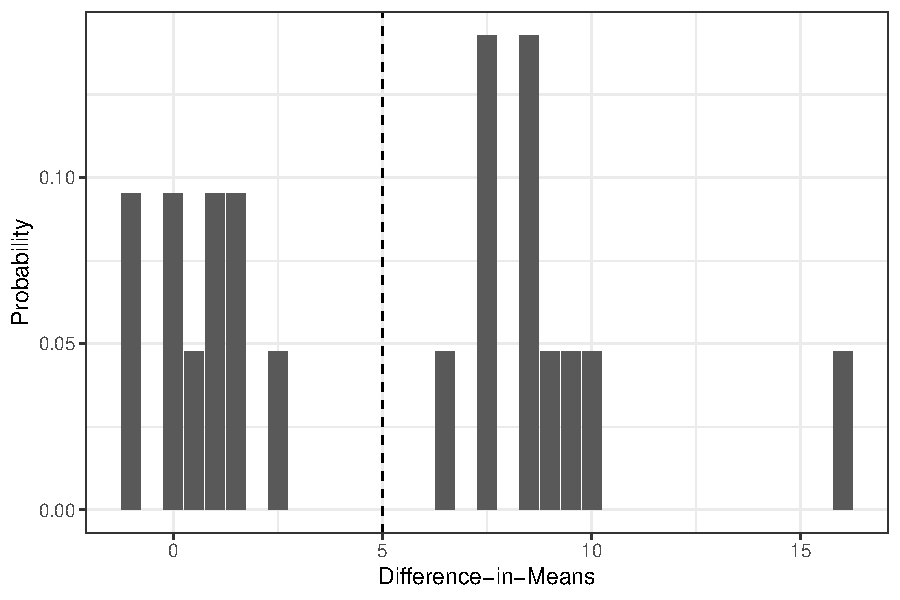
\includegraphics[width=\linewidth]{cra_est_dist_plot.pdf}
\caption{Unbiasedness of Difference-in-Means estimator in ``Village heads'' example from Gerber and Green}
\end{figure}
\end{itemize}
\end{frame}
%------------------------------------------------------------------------
\begin{frame}{Unbiasedness of Difference-in-Means estimator}
\frametitle{}
Under simple randomization, $Z_{1}, Z_{2}, \ldots, Z_{n}$ satisfy
$\Pr(Z_{i} =1) = \Pr(Z_{j} = 1)$, but $\mathbf{Z}'\mathbf{1}$ and $\left(\mathbf{1} - \mathbf{Z}\right)'\mathbf{1}$ can vary. In consequence, in general
\begin{align*}
\E\left[\frac{\mathbf{Z}'\mathbf{Y}}{\mathbf{Z}'\mathbf{1}} \right] \neq
\frac{\E[ \mathbf{Z}'\mathbf{Y} ]}{\E[ \mathbf{Z}'\mathbf{1} ]} \text{ and } \E\left[\frac{\left(\mathbf{1} - \mathbf{Z}\right)'\mathbf{Y}}{\left(\mathbf{1} - \mathbf{Z}\right)'\mathbf{1}} \right] \neq
\frac{\E[ \left(\mathbf{1} - \mathbf{Z}\right)'\mathbf{Y} ]}{\E[ \left(\mathbf{1} - \mathbf{Z}\right)'\mathbf{1} ]}
\end{align*}
 So principle unbiasedness of Difference-in-Means estimator does not
 immediately carry over from completely randomized designs.
\pause
However:
  \begin{itemize}
  \item $\mathbf{Z}'\mathbf{Y} = \mathbf{Z}'\mathbf{y_t}$ and $\left(\mathbf{1} - \mathbf{Z}\right)'\mathbf{Y} = \mathbf{Z}'\mathbf{y_c}$;
\item $\E\left[\frac{\mathbf{Z}'\mathbf{y}_{T}}{\mathbf{Z}'\mathbf{1}}\big | \mathbf{Z}'\mathbf{1} =n_{1}\right] = \bar{y}_t$, for all $n_1: n_{1} \neq 0$
\item $\E\left[\frac{\left(\mathbf{1} - \mathbf{Z}\right)'\mathbf{y}_{c}}{\left(\mathbf{1} - \mathbf{Z}\right)'\mathbf{1}}\big | \left(\mathbf{1} - \mathbf{Z}\right)'\mathbf{1} = n_{0}\right] = \bar{y}_c$, for all $n_0: n_{0} \neq 0$
  \end{itemize}


\end{frame}
%------------------------------------------------------------------------
\section{Consistency of Difference-in-Means estimator}
\begin{frame}{Consistency}
\begin{itemize}
\item Consistency is an asymptotic property
\item Consider the following conception of asymptotic growth (Brewer, 1979; Middleton and Aronow, 2015):
\begin{enumerate}
\item The original population of $n$ units is copied $h − 1$ times 
\item Within each of the $h$ copies, the assignment process is the same as in the original experiment, e.g., under CRA exactly $n_1$ units are assigned to the treatment condition and the remaining $n_0 = n − n_1$ units are assigned to the control condition
\item The $h$ copies are then collected into a single population with $hn$ total units, $hn_1$ treated units and $hn_0$ control units.
\end{enumerate}  
\end{itemize}
\end{frame}
%------------------------------------------------------------------------
\begin{frame}{``Village heads'' asymptotic growth}
\begin{table}[H]
\scriptsize
\centering
\begin{tabular}{l|l|l}
$\mathbf{y_c}$ & $\mathbf{y_t}$ & $\pmb{\tau}$ \\ \midrule
10  & 15 &  5 \\
15  & 15 &  0 \\
20  & 30 &  10 \\
20  & 15 &  -5\\
10  & 20 &  10 \\
15  & 15 &  0 \\
15  & 30 &  15
\end{tabular}
\hfill
\begin{tabular}{l|l|l}
$\mathbf{y_c}$ & $\mathbf{y_t}$ & $\pmb{\tau}$ \\ \midrule
10  & 15 &  5 \\
15  & 15 &  0 \\
20  & 30 &  10 \\
20  & 15 &  -5\\
10  & 20 &  10 \\
15  & 15 &  0 \\
15  & 30 &  15 \\ \midrule
10  & 15 &  5 \\
15  & 15 &  0 \\
20  & 30 &  10 \\
20  & 15 &  -5\\
10  & 20 &  10 \\
15  & 15 &  0 \\
15  & 30 &  15
\end{tabular}
\hfill
\begin{tabular}{l|l|l}
$\mathbf{y_c}$ & $\mathbf{y_t}$ & $\pmb{\tau}$ \\ \midrule
10  & 15 &  5 \\
15  & 15 &  0 \\
20  & 30 &  10 \\
20  & 15 &  -5\\
10  & 20 &  10 \\
15  & 15 &  0 \\
15  & 30 &  15 \\ \midrule
10  & 15 &  5 \\
15  & 15 &  0 \\
20  & 30 &  10 \\
20  & 15 &  -5\\
10  & 20 &  10 \\
15  & 15 &  0 \\
15  & 30 &  15 \\ \midrule
10  & 15 &  5 \\
15  & 15 &  0 \\
20  & 30 &  10 \\
20  & 15 &  -5\\
10  & 20 &  10 \\
15  & 15 &  0 \\
15  & 30 &  15
\end{tabular}
$\cdots$
\caption{Finite populations under asymptotic growth in which $h \in \left\{1, 2, 3, \ldots \right\}$}
\label{tab: asymp growth}
\end{table}

\end{frame}
%------------------------------------------------------------------------
\begin{frame}{Consistency}
\begin{itemize}
\item Consistency states that as the number of units in the study increases asymptotically, holding all other factors constant, the probability distribution of an estimator concentrates increasingly around the truth
\begin{itemize}
\item I.e., for any fixed $\varepsilon > 0$, the probability that the estimate and its target differ by no more than $\varepsilon$ tends to $1$.
\end{itemize}
\item Mathematically, 
\begin{equation}
\lim_{h \to \infty} \Pr\left(\left\lvert \hat{\bar{\tau}}\left(\mathbf{Z}, \mathbf{Y}\right) - \bar{\tau} \right\rvert < \varepsilon \right) = 1 \text{ for all } \varepsilon > 0
\end{equation}
or equivalently
\begin{equation}
\lim_{h \to \infty} \Pr\left(\hat{\bar{\tau}}\left(\mathbf{Z}, \mathbf{Y}\right) \in \left(\bar{\tau} - \varepsilon, \bar{\tau} + \varepsilon\right)\right) = 1 \text{ for all } \varepsilon > 0
\end{equation}
\end{itemize}
\end{frame}
%------------------------------------------------------------------------
\begin{frame}{Consistency of Difference-in-Means estimator}
\begin{itemize}
\item Estimator under complete random assignment and asymptotic growth described on prior slides:
\item[] 
\begin{figure}[H]
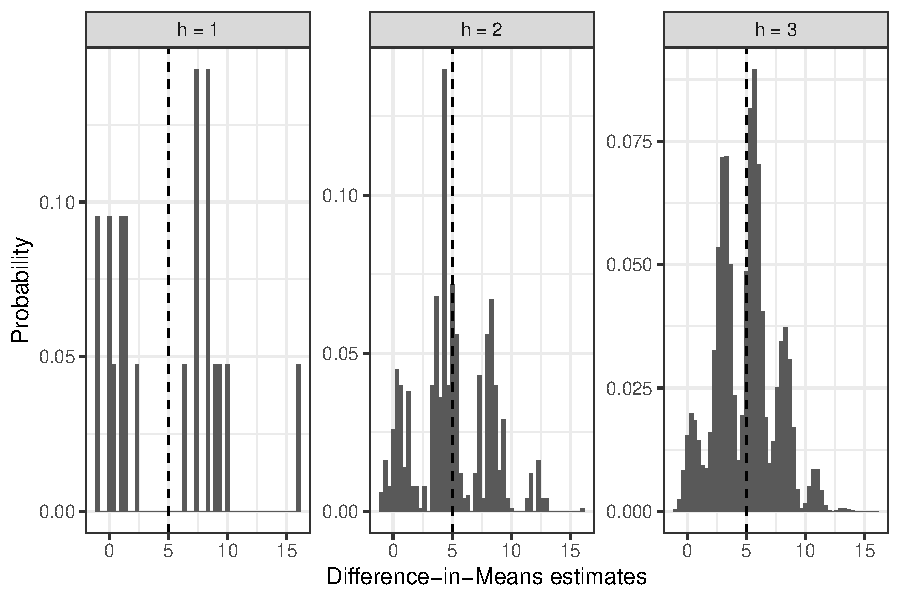
\includegraphics[width=0.95\linewidth]{asymp_ests_plot.pdf}
\caption{Consistency of Difference-in-Means estimator in ``Village heads'' example from Gerber and Green}
\end{figure}
\end{itemize}
\end{frame}
%------------------------------------------------------------------------
\end{document}